%% Full framework figure (journal / robustidps.ai platform version): the seven
%% modules of fig1_LipMamba_arch.png with the corrected mathematics.
%% Standalone-compilable: pdflatex fig1_platform.tex
\documentclass[tikz,border=4pt]{standalone}
\usepackage{amsmath,amssymb,bm}
\usetikzlibrary{positioning,fit,calc,backgrounds,arrows.meta}
\newcommand{\norm}[1]{\left\lVert #1\right\rVert}
\newcommand{\softplus}{\mathrm{softplus}}
\newcommand{\SiLU}{\mathrm{SiLU}}
\newcommand{\diag}{\mathrm{diag}}
\newcommand{\Abar}{\bar{\mathbf{A}}}
\newcommand{\h}{\mathbf{h}}
\newcommand{\x}{\mathbf{x}}
\begin{document}
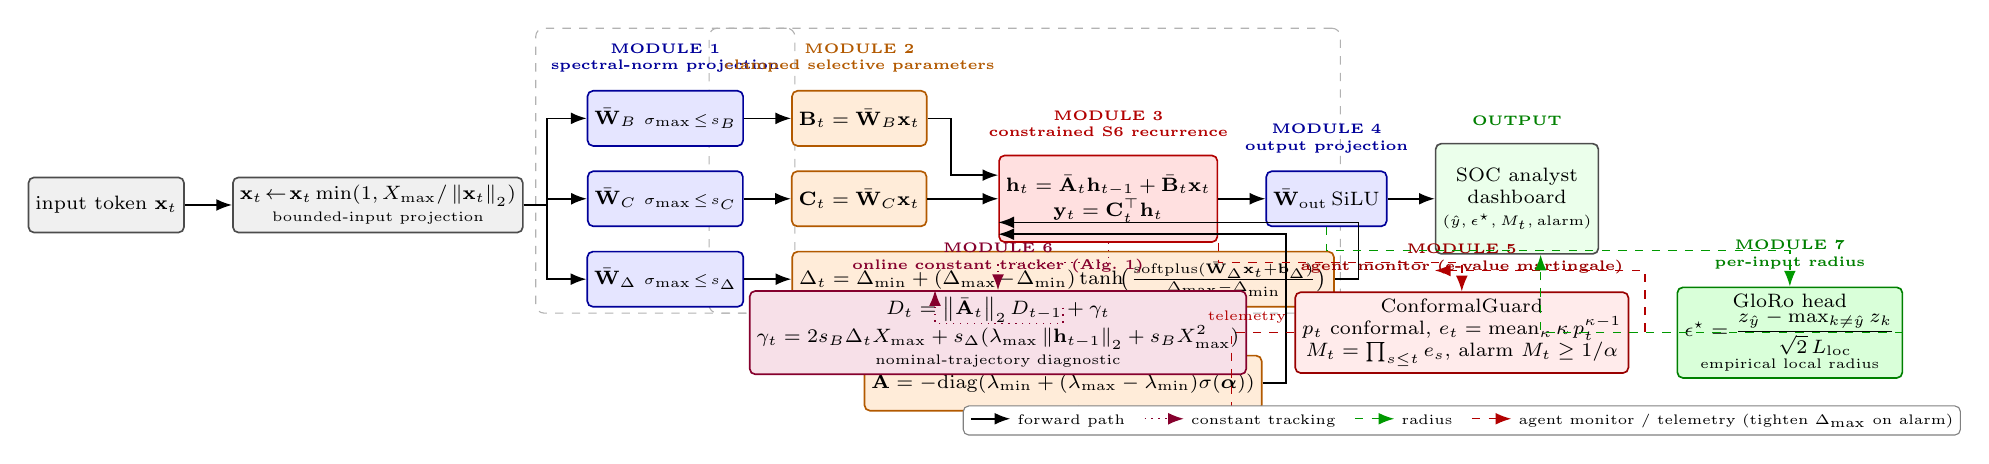
\begin{tikzpicture}[
    font=\scriptsize,
    box/.style={draw, rounded corners=2pt, minimum height=7mm, align=center, line width=0.6pt, inner sep=2.5pt},
    proj/.style={box, fill=blue!10, draw=blue!60!black},
    constraint/.style={box, fill=orange!15, draw=orange!70!black},
    ssm/.style={box, fill=red!12, draw=red!70!black, minimum height=11mm},
    cert/.style={box, fill=green!15, draw=green!50!black},
    track/.style={box, fill=purple!12, draw=purple!70!black},
    mon/.style={box, fill=red!8, draw=red!60!black},
    io/.style={box, fill=gray!12, draw=gray!60!black},
    arrow/.style={-{Latex[length=2mm]}, line width=0.6pt},
    cflow/.style={-{Latex[length=2mm]}, line width=0.5pt, dashed, draw=green!60!black},
    sflow/.style={-{Latex[length=2mm]}, line width=0.5pt, dotted, draw=purple!70!black},
    mflow/.style={-{Latex[length=2mm]}, line width=0.5pt, dashed, draw=red!70!black},
    modtitle/.style={font=\tiny\bfseries, align=center},
    bigbox/.style={draw=black!30, dashed, rounded corners=3pt, line width=0.4pt, inner sep=2pt},
    node distance=3mm and 6mm,
]
\node[io] (xt) {input token $\x_t$};
\node[io, right=of xt] (proj) {$\x_t\!\leftarrow\!\x_t\min(1,X_{\max}/\norm{\x_t}_2)$\\ \tiny bounded-input projection};
\node[proj, right=8mm of proj, yshift=11mm] (WB) {$\bar{\mathbf W}_B$ \tiny$\sigma_{\max}\!\le\!s_B$};
\node[proj, below=of WB] (WC) {$\bar{\mathbf W}_C$ \tiny$\sigma_{\max}\!\le\!s_C$};
\node[proj, below=of WC] (WD) {$\bar{\mathbf W}_\Delta$ \tiny$\sigma_{\max}\!\le\!s_\Delta$};
\node[modtitle, above=1mm of WB, text=blue!60!black] (t1) {MODULE 1\\spectral-norm projection};
\begin{scope}[on background layer]\node[bigbox, fit=(WB)(WC)(WD)(t1)] {};\end{scope}
\node[constraint, right=of WB] (Bt) {$\mathbf B_t=\bar{\mathbf W}_B\x_t$};
\node[constraint, right=of WC] (Ct) {$\mathbf C_t=\bar{\mathbf W}_C\x_t$};
\node[constraint, right=of WD] (Dt) {$\Delta_t=\Delta_{\min}+(\Delta_{\max}\!-\!\Delta_{\min})\tanh\!\bigl(\tfrac{\softplus(\bar{\mathbf W}_\Delta\x_t+\mathbf b_\Delta)}{\Delta_{\max}-\Delta_{\min}}\bigr)$};
\node[modtitle, above=1mm of Bt, text=orange!70!black] (t2) {MODULE 2\\clamped selective parameters};
\begin{scope}[on background layer]\node[bigbox, fit=(Bt)(Ct)(Dt)(t2)] {};\end{scope}
\node[constraint, below=6mm of Dt] (Aeig) {$\mathbf A=-\diag(\lambda_{\min}+(\lambda_{\max}-\lambda_{\min})\sigma(\bm\alpha))$};
\node[ssm, right=9mm of Ct] (scan) {$\h_t=\Abar_t\h_{t-1}+\bar{\mathbf B}_t\x_t$\\ $\mathbf y_t=\mathbf C_t^\top\h_t$};
\node[modtitle, above=1mm of scan, text=red!70!black] {MODULE 3\\constrained S6 recurrence};
\node[proj, right=of scan] (Wout) {$\bar{\mathbf W}_{\mathrm{out}}\,\SiLU$};
\node[modtitle, above=1mm of Wout, text=blue!60!black] {MODULE 4\\output projection};
\node[io, right=of Wout, fill=green!8, minimum height=14mm] (dash) {SOC analyst\\dashboard\\ \tiny$(\hat y,\epsilon^\star,M_t,\text{alarm})$};
\node[modtitle, above=1mm of dash, text=green!50!black] {OUTPUT};

\node[track, below=6mm of scan, xshift=-14mm] (Dtrk) {$D_t=\norm{\Abar_t}_2D_{t-1}+\gamma_t$\\ $\gamma_t=2s_B\Delta_tX_{\max}+s_\Delta(\lambda_{\max}\norm{\h_{t-1}}_2+s_BX_{\max}^2)$\\ \tiny nominal-trajectory diagnostic};
\node[modtitle, above=1mm of Dtrk, text=purple!70!black] {MODULE 6\\online constant tracker (Alg.~1)};
\node[mon, right=of Dtrk] (guard) {ConformalGuard\\ $p_t$ conformal, $e_t=\mathrm{mean}_\kappa\,\kappa\,p_t^{\kappa-1}$\\ $M_t=\prod_{s\le t}e_s$, alarm $M_t\ge1/\alpha$};
\node[modtitle, above=1mm of guard, text=red!60!black] {MODULE 5\\agent monitor (e-value martingale)};
\node[cert, right=of guard] (head) {GloRo head\\ $\epsilon^\star=\dfrac{z_{\hat y}-\max_{k\ne\hat y}z_k}{\sqrt2\,L_{\mathrm{loc}}}$\\ \tiny empirical local radius};
\node[modtitle, above=1mm of head, text=green!50!black] {MODULE 7\\per-input radius};

\draw[arrow] (xt) -- (proj);
\draw[arrow] (proj.east) -- ++(3mm,0) |- (WB.west);
\draw[arrow] (proj.east) -- ++(3mm,0) |- (WC.west);
\draw[arrow] (proj.east) -- ++(3mm,0) |- (WD.west);
\draw[arrow] (WB) -- (Bt); \draw[arrow] (WC) -- (Ct); \draw[arrow] (WD) -- (Dt);
\draw[arrow] (Bt.east) -- ++(3mm,0) |- ([yshift=3mm]scan.west);
\draw[arrow] (Ct.east) -- (scan.west);
\draw[arrow] (Dt.east) -- ++(3mm,0) |- ([yshift=-3mm]scan.west);
\draw[arrow] (Aeig.east) -- ++(3mm,0) |- ([yshift=-4.5mm]scan.west);
\draw[arrow] (scan) -- (Wout); \draw[arrow] (Wout) -- (dash);
\draw[sflow] (scan.south) -- ++(0,-2.5mm) -| (Dtrk.north);
\draw[sflow] (Dt.south) -- ++(0,-2mm) -| ([xshift=-8mm]Dtrk.north);
\draw[mflow] (scan.south east) -- ++(0,-2.5mm) -| (guard.north);
\draw[mflow] (guard.west) -- ++(-2mm,0) node[above, font=\tiny, text=red!70!black, xshift=-4mm] {telemetry} |- ++(-6mm,0) |- (Aeig.south);
\draw[mflow] (guard.east) -- ++(2mm,0) |- ([yshift=-2mm]dash.south west);
\draw[cflow] (Wout.south) -- ++(0,-3mm) -| (head.north);
\draw[cflow] (head.east) -| ([xshift=3mm]dash.south);
\node[draw=black!50, rounded corners=2pt, line width=0.4pt, fill=white, below=4mm of guard, font=\tiny, align=left, inner sep=2.5pt] {%
\tikz\draw[arrow] (0,0)--(0.5,0); forward path\quad
\tikz\draw[sflow] (0,0)--(0.5,0); constant tracking\quad
\tikz\draw[cflow] (0,0)--(0.5,0); radius\quad
\tikz\draw[mflow] (0,0)--(0.5,0); agent monitor / telemetry (tighten $\Delta_{\max}$ on alarm)};
\end{tikzpicture}
\end{document}
